% RLC-Serienschwingkreis - ImpedanXkurve |Z|,R,|X|,|X_L|,|X_C| von w/w0
\def\R{10}%     10 Ohm
\def\L{10e-3}%  10 mH
\def\C{10e-6}%  10 uF
\def\Xk{31.623}% Xk = sqrt(L/C) = 31.623 Ohm
% w0 = 1/sqrt(LC) = 3162.278 Hz
% Güte Q = Xk/R -> R = Xk/Q
% TODO: Adjust order of plotting vs order of legend, Ref: https://tex.stackexchange.com/questions/375074/ordering-of-legend-vs-zorder
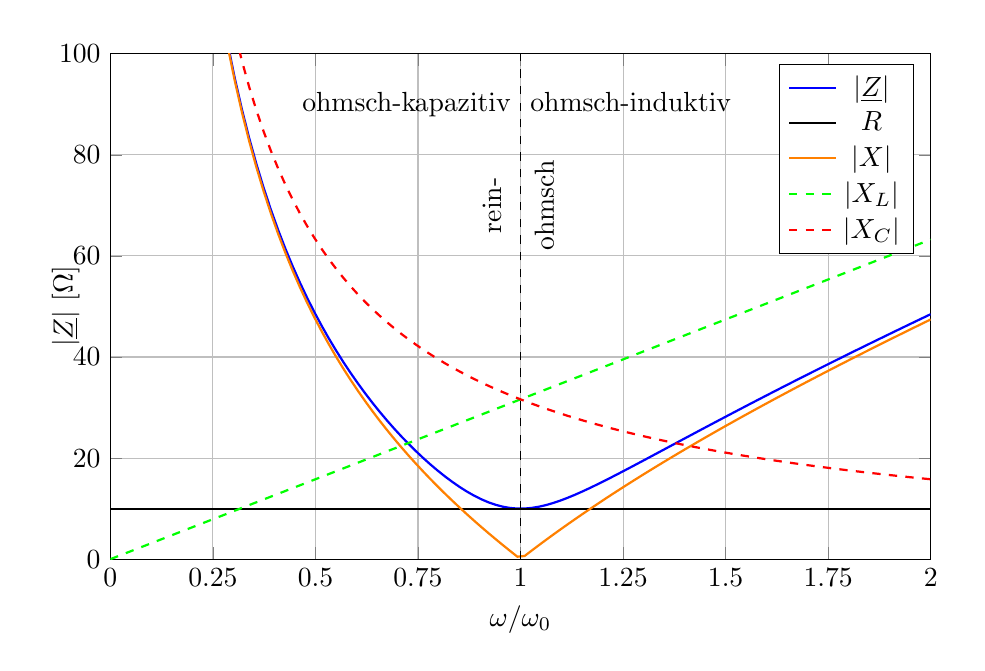
\begin{tikzpicture}[x=1cm,y=1cm]
    \draw[draw=none] (-1.05,-1) rectangle (10.75,6.75); % boundbox (not matching width and height, don't know why)
    \begin{axis}[
        xlabel={$\omega/\omega_0$},
        ylabel={$|\underline{Z}|\ [\Omega]$},
        ylabel style={yshift=-0.5cm},
        xmin=0, xmax=2,
        ymin=0, ymax=100,
        width=12cm,
        height=8cm,
        samples=100,
        xtick={0, 0.25, 0.5, 0.75, 1, 1.25, 1.5, 1.75,2},
        grid=both,
        mark=none,
    ]
    % Z = R + jX = R + j(X_L+X_C) = R + j*Xk*(w/w0 - w0/w)
    % |Z| = sqrt(R^2+X^2) = sqrt( R^2 + Xk^2*(w/w0 - w0/w)^2 )
    % R = konst.
    % |X| = |Xk*(w/w0 - w0/w)|
    % |X_L| = |Xk*(w/w0)|
    % |X_C| = |Xk*(w0/w)|
\addplot[domain=0.25:2, thick, color=blue]          {( \R^2 + \Xk^2*(x-1/x)^2 )^0.5}; % |Z|
\addplot[domain=0.00:2, thick, color=black]         {\R}; % R
\addplot[domain=0.25:2, thick, color=orange]        {abs( \Xk*(x-1/x) )}; % |X|
\addplot[domain=0.00:2, thick, color=green,dashed]  {abs( \Xk*(x) )}; % |X_L|
\addplot[domain=0.25:2, thick, color=red,dashed]    {abs( \Xk*(1/x) )}; % |X_C|
\addlegendentry{$|\underline{Z}|$}
\addlegendentry{$R$}
\addlegendentry{$|X|$}
\addlegendentry{$|X_L|$}
\addlegendentry{$|X_C|$}
% w0 Grenze (Fallunterscheidung)
\addplot[color=black, dashed, mark=none] coordinates {(1,0)(1,100)};% Warning: Missing character: There is no . 0 1 p t in font nullfont!
\node at (axis cs:1,70)[rotate=90,above]{rein-$\vphantom{\big|}$};
\node at (axis cs:1,70)[rotate=90,below]{ohmsch$\vphantom{\big|}$};
\node at (axis cs:1,90)[black,left]{ohmsch-kapazitiv$\vphantom{\big|}$};
\node at (axis cs:1,90)[black,right]{ohmsch-induktiv$\vphantom{\big|}$};
\end{axis}
\end{tikzpicture}